\chapter{Introduction}

\section{Introduction}
In written text, each person has a unique style of writing similar to a fingerprint, and in order to identify that writing style linguists have devised methods and researched features that allows those styles to be differentiated and identified from one another.

\subsection{Background}
Stylometry is the statistical methods used to analyze and differentiate between different literary styles between one author and another. A stylometric analysis is be conducted using NLP techniques and libraries due to the large and extensive tool set and previous research and applications achieved.

\subsection{Motivation}
The process of identifying a writing's features is a difficult task that involves excessive manual labor and time analyzing each sentence and clause several times to extract all of the features.

\subsection{Problem Definitions}
The main problems are:
\begin{itemize}
  \item Converting the stylometric features to machine readable form.
  \item Applying those features with NLP techniques for analysis.
  \item Providing a functional interface that allows for complete utilization of the system and its features.
\end{itemize}

\section{Project Description}

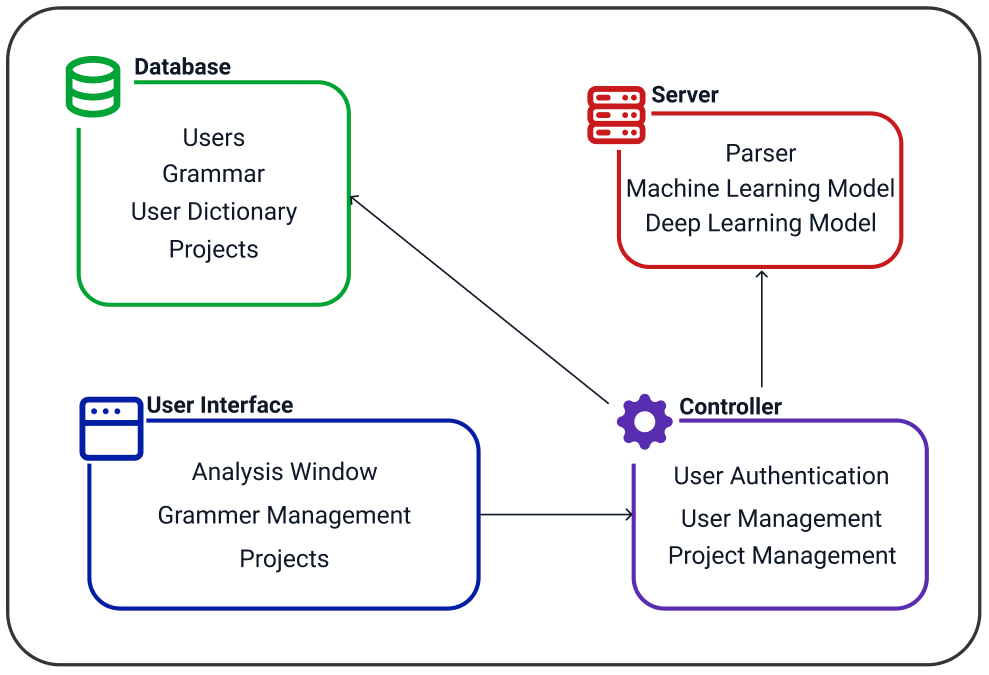
\includegraphics[width=10cm]{images/System Overview.png}

\subsection{Scope}
The scope of the project lies is limited to NLP, text analysis, and statistical operations.

\subsection{Project Overview}
\begin{itemize}
  \item Document and project storage.
  \item Analysis server.
  \item User interface.
\end{itemize}
